% !TEX TS-program = pdflatex
% !TEX encoding = UTF-8 Unicode

% This is a simple template for a LaTeX document using the "article" class.
% See "book", "report", "letter" for other types of document.

\documentclass[11pt]{article} % use larger type; default would be 10pt

\usepackage[utf8]{inputenc} % set input encoding (not needed with XeLaTeX)

%%% Examples of Article customizations
% These packages are optional, depending whether you want the features they provide.
% See the LaTeX Companion or other references for full information.

%%% PAGE DIMENSIONS
\usepackage{geometry} % to change the page dimensions
\geometry{a4paper} % or letterpaper (US) or a5paper or....
\geometry{margin=1in} % for example, change the margins to 2 inches all round
% \geometry{landscape} % set up the page for landscape
%   read geometry.pdf for detailed page layout information

\usepackage{graphicx} % support the \includegraphics command and options

% \usepackage[parfill]{parskip} % Activate to begin paragraphs with an empty line rather than an indent
\usepackage{amssymb}
\usepackage{amsmath}
%%% PACKAGES
\usepackage{booktabs} % for much better looking tables
\usepackage{array} % for better arrays (eg matrices) in maths
\usepackage{paralist} % very flexible & customisable lists (eg. enumerate/itemize, etc.)
\usepackage{verbatim} % adds environment for commenting out blocks of text & for better verbatim
\usepackage{subfig} % make it possible to include more than one captioned figure/table in a single float
% These packages are all incorporated in the memoir class to one degree or another...

%%% HEADERS & FOOTERS
\usepackage{fancyhdr} % This should be set AFTER setting up the page geometry
\pagestyle{fancy} % options: empty , plain , fancy
\renewcommand{\headrulewidth}{0pt} % customise the layout...
\lhead{}\chead{}\rhead{}
\lfoot{}\cfoot{\thepage}\rfoot{}

%%% SECTION TITLE APPEARANCE
\usepackage{sectsty}
\allsectionsfont{\sffamily\mdseries\upshape} % (See the fntguide.pdf for font help)
% (This matches ConTeXt defaults)

%%% ToC (table of contents) APPEARANCE
\usepackage[nottoc,notlof,notlot]{tocbibind} % Put the bibliography in the ToC
\usepackage[titles,subfigure]{tocloft} % Alter the style of the Table of Contents
\usepackage{bbm}
\usepackage{endnotes}

\renewcommand{\cftsecfont}{\rmfamily\mdseries\upshape}
\renewcommand{\cftsecpagefont}{\rmfamily\mdseries\upshape} % No bold!
\DeclareMathOperator*{\argmax}{arg\,max}
\DeclareMathOperator*{\argmin}{arg\,min}

\usepackage{graphicx}
\graphicspath{ {./pings/} }

\newcount\colveccount
\newcommand*\colvec[1]{
        \global\colveccount#1
        \begin{pmatrix}
        \colvecnext
}
\def\colvecnext#1{
        #1
        \global\advance\colveccount-1
        \ifnum\colveccount>0
                \\
                \expandafter\colvecnext
        \else
                \end{pmatrix}
        \fi
}

\newcommand{\norm}[1]{\left\lVert#1\right\rVert}

\title{Computational Problem Set 1}
\author{Michael B. Nattinger}

\begin{document}
\maketitle

\section{State the dynamic programming problem}
Households choose future capital levels to solve:
\begin{align*}
V(K,Z) &= \max_{K'} log(ZK^{\alpha} + (1-\delta)K - K') + \beta E_t[V(K',Z')]\\
&=  \max_{K'} log(ZK^{\alpha} + (1-\delta)K - K') + \\ &+ \beta[V(K',Z')P(Z' = Z^g|Z) + V(K',Z^b)P(Z' = Z^b|Z)]
\end{align*}

We will proceed to solve in Matlab, Julia, Fortran, and parallelized Fortran, as instructed.

Matlab results: Runtime is 18 seconds (not including figure making). Capital grid was extended to 75 from 45, and has 1000 elements. In Julia, computation is substantially quicker and convergence was achieved in 2.6 seconds to solve the same problem. Note: this is with difference computed as the sup norm of value function changes, and not normalized to the scale of value function, rather absolute size with a tolerance of $10^{-4}$. Fortran runs in 5.8 seconds. Figures below are from Matlab solution to the stochastic problem, with a capital grid with 3000 elements instead of 1000. Figures from Julia and Fortran are identical.

Note also: Matlab code is structured very differently from the Fortran/Julia code and is not optimized for performance. I would not consider  this to be a fair comparison of the speed of Matlab; rather,  I see it as a reasonably fast baseline for sub-optimal ("naively-written") code.

\section{Value function}
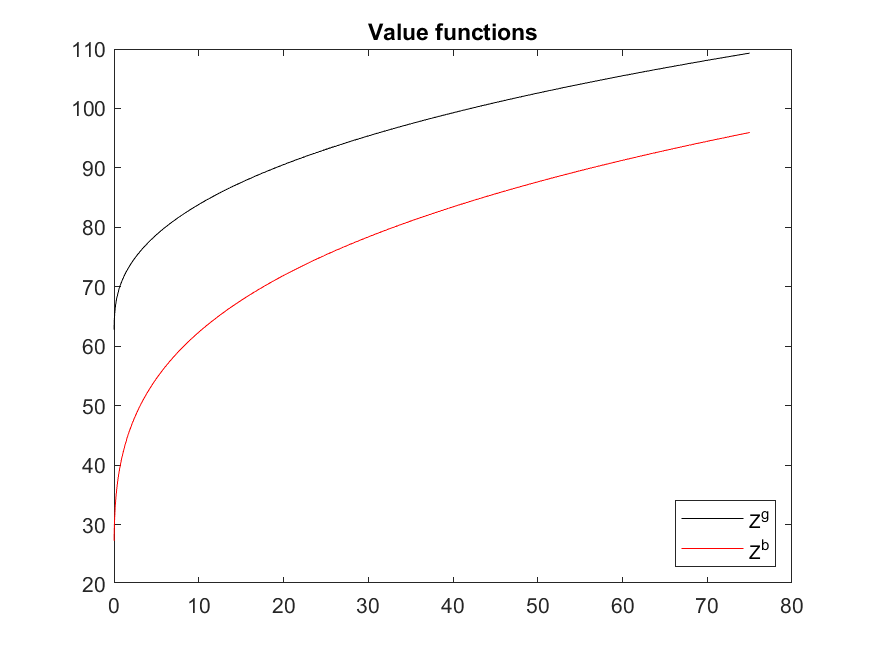
\includegraphics{value}

From the above figure, we can see that the value function is indeed increasing and concave.


\section{Decision rule}
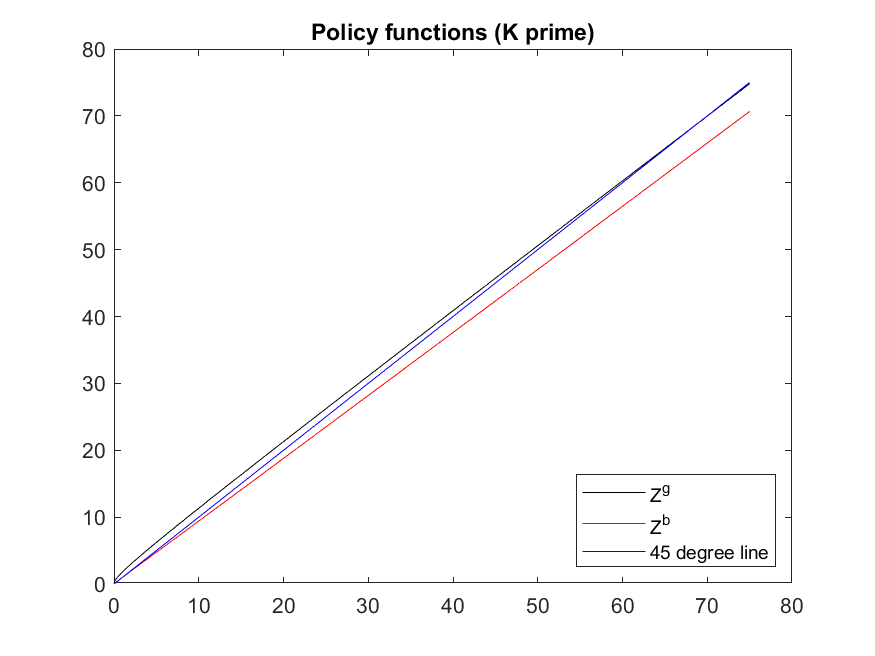
\includegraphics{policy}

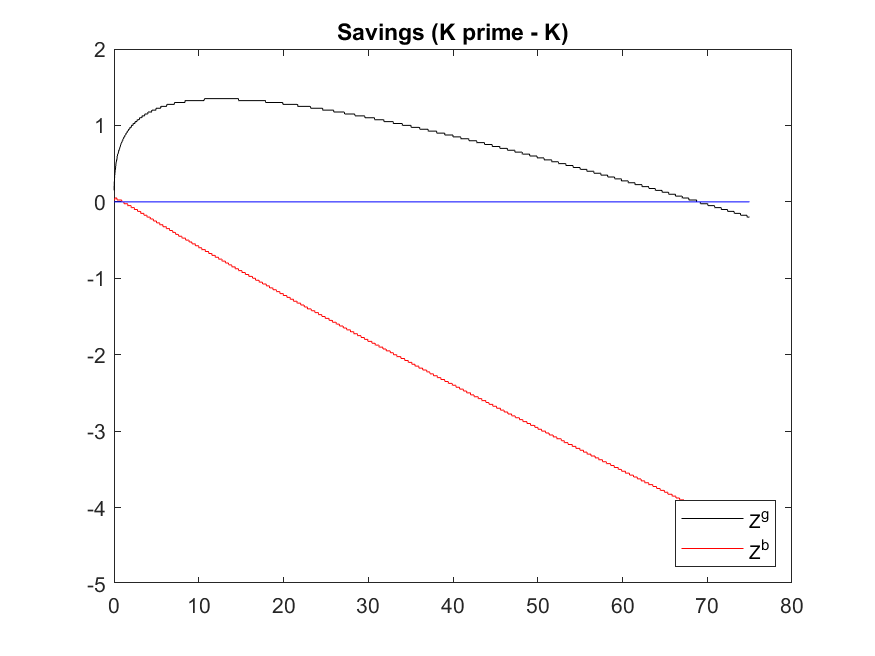
\includegraphics{savings}

From the above figures, we can see that the decision rule is increasing in K and Z. Saving is not always increasing in K - if households have sufficiently large capital levels, they are better off dissaving. However, saving is increasing in Z - under bad conditions, one will save less than they would under good conditions (conditional on K).

\end{document}
